 \documentclass[10pt]{beamer}
\usetheme[progressbar=frametitle]{metropolis}
\setbeamertemplate{mini frame}{}
\setbeamertemplate{mini frame in current section}{}
\setbeamertemplate{mini frame in current subsection}{}
\setbeamercolor{section in head/foot}{fg=normal text.bg, bg=structure.fg}
\setbeamercolor{subsection in head/foot}{fg=normal text.bg, bg=structure.fg}

\makeatletter
\setbeamertemplate{footline}{%
    \begin{beamercolorbox}[colsep=1.5pt]{upper separation line head}
    \end{beamercolorbox}
    \begin{beamercolorbox}{section in head/foot}
      \insertsubsectionnavigationhorizontal{\paperwidth}{}{\hskip0pt plus1filll}\vskip3pt%
    \end{beamercolorbox}%
    \begin{beamercolorbox}[colsep=1.5pt]{lower separation line head}
    \end{beamercolorbox}
}
\makeatother
\usepackage{appendixnumberbeamer}

\usepackage{booktabs}
\usepackage[scale=2]{ccicons}

\usepackage{pgfplots}
\usepgfplotslibrary{dateplot}

\usepackage{xspace}
\newcommand{\themename}{\textbf{\textsc{metropolis}}\xspace}

\usepackage{graphicx}
\graphicspath{ {./images/} }

\title{Introduzione alla biostatistica}
\subtitle{Corso base per ricercatori coinvolti nell'utilizzo di animali ai fini scientifici ed educativi}
% \date{\today}
\date{}
\author{Massimo Tranquillo\\
Medico Veterinario- Specialista in Statistica Medica ed Epidemiologia Clinica}
\institute{IZSLER-Sez. di Bergamo}
\titlegraphic{\hfill\includegraphics[scale=0.30]{images/logo.png}}

\begin{document}
\maketitle

\begin{frame}{Indice}
  \setbeamertemplate{section in toc}[sections numbered]
  \tableofcontents[hideallsubsections]
\end{frame}

\section{Introduzione}
%\subsection{crisi di riproducibilit�}

\subsection{cos'� la biostatistica}
\begin{frame}[fragile]{Biostatistica}
\begin{center}
    \textbf{misurare} e \textbf{spiegare} la variabilit� di fenomeni biologici
\end{center}

 \begin{figure}[h]
\includegraphics[width=8cm,height=7cm]{images/peso.png}}
\centering
\end{figure}
\end{frame}
\begin{frame}{Biostatistica}
\textbf{predire} eventi futuri!
\begin{itemize}[<+- | alert@+>]
    \item[]
    \item[] costruendo un \textbf{modello} del fenomeno biologico utilizzando i dati osservati
   \begin{center}
       \item[] $y=\alpha+ \beta \cdot X+\varepsilon$
   \end{center}
    
\end{itemize}
\end{frame}
\section{Concetti}
\subsection{modelli}
\begin{frame}{Modelli predittivi}
\begin{center}
    la media come modello predittivo
\end{center}

 \begin{center}
 \includegraphics[scale=0.30]{peso.png}
 \end{center}
 \begin{center}
   \alert{$y=\mu+\varepsilon$}
 \end{center}
 \end{frame}

\begin{frame}{$y=\mu+\varepsilon$}
 \begin{table}[H]
  \begin{center}
  \begin{tabular}{lrr}\hline\hline
 \multicolumn{1}{l}{soggetto}&
 \multicolumn{1}{c}{peso osservato}&
 \multicolumn{1}{c}{peso predetto}
 \\ \hline
 1&$1060.71$&$1011.03$\\
 2&$1009.84$&$1011.03$\\
 3&$ 721.66$&$1011.03$\\
 4&$ 882.88$&$1011.03$\\
 5&$1208.20$&$1011.03$\\
 6&$ 890.98$&$1011.03$\\
 7&$ 840.91$&$1011.03$\\
 8&$1209.05$&$1011.03$\\
 9&$1350.41$&$1011.03$\\
 10&$ 935.69$&$1011.03$\\
 \hline
 \end{tabular}
 
 \end{center}
 
 \end{table}
\end{frame}



 \begin{frame}{$y=\mu+\varepsilon$}
   \begin{table}[H]
  \begin{center}
  \begin{tabular}{lrrr}\hline\hline
 \multicolumn{1}{l}{soggetti}&
 \multicolumn{1}{c}{peso osservato}&
 \multicolumn{1}{c}{peso predetto}&
 \multicolumn{1}{c}{errore}
 \\ \hline
 1&$1060.71$&$1011.03$&$  49.68$\\
 2&$1009.84$&$1011.03$&$  -1.19$\\
 3&$ 721.66$&$1011.03$&$-289.37$\\
 4&$ 882.88$&$1011.03$&$-128.15$\\
 5&$1208.20$&$1011.03$&$ 197.17$\\
 6&$ 890.98$&$1011.03$&$-120.06$\\
 7&$ 840.91$&$1011.03$&$-170.13$\\
 8&$1209.05$&$1011.03$&$ 198.01$\\
 9&$1350.41$&$1011.03$&$ 339.38$\\
 10&$ 935.69$&$1011.03$&$ -75.34$\\
 \hline
 \end{tabular}
 \end{center}
 \end{table}
 \end{frame}


 \begin{frame}{$y=\mu+\varepsilon$}
   \begin{table}[H]
  \begin{center}
  \begin{tabular}{lrrr}\hline\hline
 \multicolumn{1}{l}{soggetti}&
 \multicolumn{1}{c}{peso osservato}&
 \multicolumn{1}{c}{peso predetto}&
 \multicolumn{1}{c}{errore}
 \\ \hline
 1&$1060.71$&$1011.03$&$  49.68$\\
 2&$1009.84$&$1011.03$&$  -1.19$\\
 3&$ 721.66$&$1011.03$&$-289.37$\\
 4&$ 882.88$&$1011.03$&$-128.15$\\
 5&$1208.20$&$1011.03$&$ 197.17$\\
 6&$ 890.98$&$1011.03$&$-120.06$\\
 7&$ 840.91$&$1011.03$&$-170.13$\\
 8&$1209.05$&$1011.03$&$ 198.01$\\
 9&$1350.41$&$1011.03$&$ 339.38$\\
 10&$ 935.69$&$1011.03$&$ -75.34$\\
 \hline
 somma degli errori&$ $&$ $&$0$\\
 \hline
 \end{tabular}
 \end{center}
 \end{table}
 \end{frame}

 \begin{frame}{$y=\mu+\varepsilon$}
   \begin{table}[H]
  \begin{center}
  \begin{tabular}{lrrr}\hline\hline
 \multicolumn{1}{l}{soggetti}&
 \multicolumn{1}{c}{peso osservato}&
 \multicolumn{1}{c}{peso predetto}&
 \multicolumn{1}{c}{errore}
 \\ \hline
 1&$1060.71$&$1011.03$&$  49.68$\\
 2&$1009.84$&$1011.03$&$  -1.19$\\
 3&$ 721.66$&$1011.03$&$-289.37$\\
 4&$ 882.88$&$1011.03$&$-128.15$\\
 5&$1208.20$&$1011.03$&$ 197.17$\\
 6&$ 890.98$&$1011.03$&$-120.06$\\
 7&$ 840.91$&$1011.03$&$-170.13$\\
 8&$1209.05$&$1011.03$&$ 198.01$\\
 9&$1350.41$&$1011.03$&$ 339.38$\\
 10&$ 935.69$&$1011.03$&$ -75.34$\\
 \hline
 somma degli errori&$ $&$ $&$0$\\
 \hline
 somma dei quadrati&$ $&$ $&$38324.94$\\
 \hline
 \end{tabular}
 \end{center}
 \end{table}
 \end{frame}


 \begin{frame}{$y=\mu+\varepsilon$}
   \begin{table}[H]
  \begin{center}
  \begin{tabular}{lrrr}\hline\hline
 \multicolumn{1}{l}{soggetti}&
 \multicolumn{1}{c}{peso osservato}&
 \multicolumn{1}{c}{peso predetto}&
 \multicolumn{1}{c}{errore}
 \\ \hline
 1&$1060.71$&$1011.03$&$  49.68$\\
 2&$1009.84$&$1011.03$&$  -1.19$\\
 3&$ 721.66$&$1011.03$&$-289.37$\\
 4&$ 882.88$&$1011.03$&$-128.15$\\
 5&$1208.20$&$1011.03$&$ 197.17$\\
 6&$ 890.98$&$1011.03$&$-120.06$\\
 7&$ 840.91$&$1011.03$&$-170.13$\\
 8&$1209.05$&$1011.03$&$ 198.01$\\
 9&$1350.41$&$1011.03$&$ 339.38$\\
 10&$ 935.69$&$1011.03$&$ -75.34$\\
 \hline
 somma degli errori&$ $&$ $&$0$\\
 \hline
 somma dei quadrati&$ $&$ $&$38324.94$\\
 \hline
 Varianza&$ $&$ $&$3832.49$\\
 \hline
 
 \end{tabular}
 \end{center}
 \end{table}
 \end{frame}
 
 
  \begin{frame}{$y=\mu+\varepsilon$}
   \begin{table}[H]
  \begin{center}
  \begin{tabular}{lrrr}\hline\hline
 \multicolumn{1}{l}{soggetti}&
 \multicolumn{1}{c}{peso osservato}&
 \multicolumn{1}{c}{peso predetto}&
 \multicolumn{1}{c}{errore}
 \\ \hline
 1&$1060.71$&$1011.03$&$  49.68$\\
 2&$1009.84$&$1011.03$&$  -1.19$\\
 3&$ 721.66$&$1011.03$&$-289.37$\\
 4&$ 882.88$&$1011.03$&$-128.15$\\
 5&$1208.20$&$1011.03$&$ 197.17$\\
 6&$ 890.98$&$1011.03$&$-120.06$\\
 7&$ 840.91$&$1011.03$&$-170.13$\\
 8&$1209.05$&$1011.03$&$ 198.01$\\
 9&$1350.41$&$1011.03$&$ 339.38$\\
 10&$ 935.69$&$1011.03$&$ -75.34$\\
 \hline
 somma degli errori&$ $&$ $&$0$\\
 \hline
 somma dei quadrati&$ $&$ $&$38324.94$\\
 \hline
 Varianza&$ $&$ $&$3832.49$\\
 \hline
 Deviazione Standard&$ $&$ $&$61.90$\\
 \hline
 
 \end{tabular}
 \end{center}
 \end{table}
 \end{frame}

\begin{frame}{media e deviazione standard}
\begin{center}
media=1011.03 g (ds=61.90 g)
 \end{center}
\begin{center}
 \includegraphics[scale=0.30]{peso.png}
 \end{center}
\end{frame}

\begin{frame}{media e deviazione standard}

\begin{center}
 \includegraphics[scale=0.50]{images/gauss3.png}
 \end{center}
\end{frame}

\begin{frame}{media e deviazione standard}

\begin{center}
 \includegraphics[scale=0.40]{images/gauss2.png}
 \end{center}
\end{frame}


\begin{frame}{media e deviazione standard}

\begin{center}
 \includegraphics[scale=0.5]{images/area.png}
 \end{center}
\end{frame}




\begin{frame}{$y=\mu+trattamento+\varepsilon$}
 \begin{center}
     trattamento dietetico: variabile dicotomica (0=no, 1=si)
 \end{center} 
 \end{frame}
 
 \begin{frame}{$y=\mu+trattamento+\varepsilon$}
 \begin{center}
     trattamento dietetico: variabile dicotomica (0=no, 1=si)
 \end{center} 
  \begin{table}[H]
  \begin{center}
  \begin{tabular}{lrr}\hline\hline
 \multicolumn{1}{l}{soggetti}&
 \multicolumn{1}{c}{peso osservato}&
 \multicolumn{1}{c}{trattamento}
 \\ \hline
 1&$1060.71$&$1$\\
 2&$1009.84$&$1$\\
 3&$ 721.66$&$0$\\
 4&$ 882.88$&$0$\\
 5&$1208.20$&$1$\\
 6&$ 890.98$&$0$\\
 7&$ 840.91$&$0$\\
 8&$1209.05$&$1$\\
 9&$1350.41$&$1$\\
 10&$ 935.69$&$0$\\
 \hline
 \end{tabular}
 \end{center}
 \end{table}
 \end{frame}

\begin{frame}{$y=\mu+trattamento+\varepsilon$}
   \begin{block}{modello per soggetti con trattamento =0}
 \begin{itemize} [<+- | alert@+>]   
 \item []$\mu$=854.42
  \item[] $y=\mu+\varepsilon$
 \end{itemize}
   \end{block}
   \begin{block}{modello per soggetti con trattamento=1}
       \begin{itemize}[<+- | alert@+>]
       \item[] $\mu$=1167.64
        \item []$y=\mu+\varepsilon$
       \end{itemize}
   \end{block}
 \end{frame}

 
 \begin{frame}{$y=\mu+trattamento+\varepsilon$}
 \begin{table}[H]
  \begin{center}
  \begin{tabular}{lrrrr}\hline\hline
 \multicolumn{1}{l}{soggetti}&
 \multicolumn{1}{c}{peso osservato}&
 \multicolumn{1}{c}{pasto}&
 \multicolumn{1}{c}{peso predetto}&
 \multicolumn{1}{c}{errore}
 \\ \hline
 1&$1060.71$&$1$&$1167.642$&$-106.932$\\
 2&$1009.84$&$1$&$1167.642$&$-157.802$\\
 3&$ 721.66$&$0$&$ 854.424$&$-132.764$\\
 4&$ 882.88$&$0$&$ 854.424$&$  28.456$\\
 5&$1208.20$&$1$&$1167.642$&$  40.558$\\
 6&$ 890.98$&$0$&$ 854.424$&$  36.556$\\
 7&$ 840.91$&$0$&$ 854.424$&$ -13.514$\\
 8&$1209.05$&$1$&$1167.642$&$  41.408$\\
 9&$1350.41$&$1$&$1167.642$&$ 182.768$\\
 10&$ 935.69$&$0$&$ 854.424$&$  81.266$\\
 \hline
 \end{tabular}
 
 \end{center}
 
 \end{table}
 
 \end{frame}
 
 \begin{frame}{confronto tra modelli}
 \begin{table}[H]
  \begin{center}
  \begin{tabular}{lrr}\hline\hline
 \multicolumn{1}{l}{soggetto}&
 \multicolumn{1}{c}{$y=\mu+\varepsilon$}&
 \multicolumn{1}{c}{$y=\mu+trattamento+\varepsilon}
 \\ \hline
 1&$   49.68$&$ -106.93$\\
 2&$   -1.19$&$ -157.80$\\
 3&$ -289.37$&$ -132.76$\\
 4&$ -128.15$&$   28.46$\\
 5&$  197.17$&$   40.56$\\
 6&$ -120.06$&$   36.56$\\
 7&$ -170.13$&$  -13.51$\\
 8&$  198.01$&$   41.41$\\
 9&$  339.38$&$  182.77$\\
 10&$  -75.34$&$   81.27$\\
 \hline
 
 \end{tabular}
 \end{center}
 \end{table}
 \end{frame}
 
\begin{frame}{confronto tra modelli}
 \begin{table}[H]
  \begin{center}
  \begin{tabular}{lrr}\hline\hline
\multicolumn{1}{l}{soggetto}&
 \multicolumn{1}{c}{$y=\mu+\varepsilon$}&
 \multicolumn{1}{c}{$y=\mu+trattamento+\varepsilon$}
 \\ \hline
 1&$   49.68$&$ -106.93$\\
 2&$   -1.19$&$ -157.80$\\
 3&$ -289.37$&$ -132.76$\\
 4&$ -128.15$&$   28.46$\\
 5&$  197.17$&$   40.56$\\
 6&$ -120.06$&$   36.56$\\
 7&$ -170.13$&$  -13.51$\\
 8&$  198.01$&$   41.41$\\
 9&$  339.38$&$  182.77$\\
 10&$  -75.34$&$   81.27$\\
 \hline
Somma dei quadrati&$38324.94$&$11073.20$\\
 \end{tabular}
 
 \end{center}
 
 \end{table}
 
 \end{frame}
 
 
 \begin{frame}{confronto tra modelli}
 \begin{table}[H]
  \begin{center}
  \begin{tabular}{lrr}\hline\hline
\multicolumn{1}{l}{soggetto}&
 \multicolumn{1}{c}{$y=\mu+\varepsilon$}&
 \multicolumn{1}{c}{$y=\mu+trattamento+\varepsilon$}
 \\ \hline
 1&$   49.68$&$ -106.93$\\
 2&$   -1.19$&$ -157.80$\\
 3&$ -289.37$&$ -132.76$\\
 4&$ -128.15$&$   28.46$\\
 5&$  197.17$&$   40.56$\\
 6&$ -120.06$&$   36.56$\\
 7&$ -170.13$&$  -13.51$\\
 8&$  198.01$&$   41.41$\\
 9&$  339.38$&$  182.77$\\
 10&$  -75.34$&$   81.27$\\
 \hline
Somma dei quadrati&$38324.94$&$11073.20$\\
\hline
 \end{tabular}
 
 \end{center}
 
 \end{table}
 
 \end{frame}
 
 \begin{frame}{scomposizione della variabilit�}
   \begin{itemize}[<+- | alert@+>] 
   \item[]
   \item variabilit� modello nullo ($y=\mu+\varepsilon$)=38324.94
   \item variabilit� modello con fattore trattamento ($y=\mu+trattamento+\varepsilon$)=11073.20
   \item variabilit� spiegata dal fattore trattamento= 38324.94-11073.20=27251.74
   \item il fattore trattamento spiega il $\frac{27251.74}{38324.94}=71\%$ della variabilit� totale
   \item resta un 30\% circa di variabilit� \textbf{non spiegata} dal modello!
   \end{itemize}
 \end{frame}

 \begin{frame}{effetto del fattore trattamento}
   \begin{itemize}
   \item $\mu_{trattamento=0}=854.42$
   \item $\mu_{trattamento=1}=1167.642$
   \item $\mu_1-\mu_2=313.22$ \\ 
   effetto del fattore trattamento 
   \end{itemize}
 \end{frame}
 
 \begin{frame}{il modello finale}
   \begin{itemize}[<+-| alert@+>]
   \item $y=\alpha+ \beta \cdot trattamento+\varepsilon$
   \item $\alpha$ valore basale (intercetta)
   \item $\beta$ \textbf{effetto} del fattore trattamento
   \item $\varepsilon$ errore residuo
   \item[]  $$y=854.42+313.22*trattamento+\varepsilon$$
   \end{itemize}
   \end{frame}

\subsection{study design}
\begin{frame}{Disegno sperimentale}
     \begin{itemize}
         \item []Obiettivo
         \item [] ridurre la quota di variabilit� residua di \textbf{Y} individuando i fattori \textbf{X} che spieghino la maggior parte della variabilit� osservata di \textbf{Y}
         \begin{itemize}[<+- | alert@+>]
            \item[]
             \item poche variabili Y ( sarebbe meglio una!!)
             \item numerose variabili X (senza esagerare)
             
         \end{itemize}
     \end{itemize}
 \end{frame}
 
 \begin{frame}{schema di una sperimentazione}
 \begin{figure}[h]
\includegraphics[scale=0.40]{images/trial.png}
\centering
\end{figure}
 \end{frame}


\section{Metodi}
\begin{frame}{Analisi dei dati}
 \begin{block}{}
        VISUALIZZAZIONE (Grafici e Tabelle)
      \end{block}
 \begin{block}{}
 \metroset{block=fill}
        INFERENZA 
      \end{block}
    
\end{frame}
 
 \subsection{natura dei dati}
 \begin{frame}{Dati}
 \begin{center}
     sono caratteristiche osservate e registrate a livello di unit� statistica (spesso coincidente con l'unit� sperimentale)
 \end{center}
\begin{center}
        \includegraphics[scale=0.25]{variabili.png}
    \end{center}
     
 \end{frame}
 
 \begin{frame}{Potere informativo dei dati}
    \begin{center}
        \includegraphics[scale=0.25]{pinfo.png}
    \end{center}
 \end{frame}


\subsection{visualizzazione dei dati}
\begin{frame}{Visualizzazione}
\end{frame}
\subsection{inferenza}

\begin{frame}{ inferenza deduttiva e inferenza induttiva }
\begin{center}
        \includegraphics[scale=0.40]{medinf.png}
\end{center}
\end{frame}




\begin{frame}{ inferenza deduttiva e inferenza induttiva }
\begin{center}
        \includegraphics[scale=0.40]{statinf.png}
\end{center}
\end{frame}

\begin{frame}{Inferenza statistica}
\begin{itemize}
       \item METODI DEDUTTIVI
        \begin{itemize}
            \item CONFUTAZIONE DI IPOTESI
                    \begin{itemize}
            \item Test di significativit� di Fisher
            \item Test di ipotesi di Newman-Pearson
            \item Null Hypothesis Significant Test (NHST)
                     \end{itemize}
        \end{itemize}
       
       \item METODI INDUTTIVI
       \begin{itemize}
        \item LIKELIHOOD (VEROSIMIGLIANZA)
        \item TEOREMA DI BAYES 
        \end{itemize}
       
\end{itemize}
\end{frame}

\subsection{metodi deduttivi}
\begin{frame}{Test di significativit� di Fisher}

\begin{columns}
\column{0.3\textwidth}
\begin{center}
    \includegraphics[scale=0.4]{images/Fisher.jpg}
\end{center}
\begin{center}
$$P(dati|ipotesi)$$
\end{center}
\column{0.7\textwidth}
\begin{center}
    p-value
\end{center}
\begin{center}
    \includegraphics[scale=0.4]{images/pregion.png}
\end{center}
\end{columns}
\end{frame}

\begin{frame}{Test di significativit� di Fisher}
\begin{center}
    \includegraphics[scale=0.3]{images/pvalue.png}
\end{center}
\end{frame}





\begin{frame}{Test d'ipotesti di Newman-Pearson}
\begin{center}
    \includegraphics[scale=0.5]{images/FN1.PNG}
\end{center}
    
\end{frame}


\begin{frame}{Test d'ipotesti di Newman-Pearson}
\begin{center}
    \includegraphics[scale=0.5]{images/FN2.PNG}
\end{center}
    
\end{frame}

\begin{frame}{Null Hypothesis Significant Test- NHST}
    \begin{center}
    \includegraphics[scale=0.5]{images/nhst.PNG}
\end{center}
\end{frame}

\begin{frame}{Likelihood- Verosimiglianza}
\end{frame}

\begin{frame}{Likelihood}
\begin{table}[ht]
\begingroup\fontsize{8pt}{13pt}\selectfont
\begin{tabular}{rrrrrrrrrr}
  \hline
dati & P=0.1 & P=0.2 & P=0.3 & P=0.4 & P=0.5 & P=0.6 & P=0.7 & P=0.8 & P=0.9 \\ 
  \hline
0 & 0.35 & 0.11 & 0.03 & 0.01 & 0.00 & 0.00 & 0.00 & 0.00 & 0.00 \\ 
  1 & 0.39 & 0.27 & 0.12 & 0.04 & 0.01 & 0.00 & 0.00 & 0.00 & 0.00 \\ 
  2 & 0.19 & 0.30 & 0.23 & 0.12 & 0.04 & 0.01 & 0.00 & 0.00 & 0.00 \\ 
  3 & 0.06 & 0.20 & 0.27 & 0.21 & 0.12 & 0.04 & 0.01 & 0.00 & 0.00 \\ 
  4 & 0.01 & 0.09 & 0.20 & 0.25 & 0.21 & 0.11 & 0.04 & 0.01 & 0.00 \\ 
  5 & 0.00 & 0.03 & 0.10 & 0.20 & 0.25 & 0.20 & 0.10 & 0.03 & 0.00 \\ 
  6 & 0.00 & 0.01 & 0.04 & 0.11 & 0.21 & 0.25 & 0.20 & 0.09 & 0.01 \\ 
  7 & 0.00 & 0.00 & 0.01 & 0.04 & 0.12 & 0.21 & 0.27 & 0.20 & 0.06 \\ 
  8 & 0.00 & 0.00 & 0.00 & 0.01 & 0.04 & 0.12 & 0.23 & 0.30 & 0.19 \\ 
  9 & 0.00 & 0.00 & 0.00 & 0.00 & 0.01 & 0.04 & 0.12 & 0.27 & 0.39 \\ 
  10 & 0.00 & 0.00 & 0.00 & 0.00 & 0.00 & 0.01 & 0.03 & 0.11 & 0.35 \\ 
   \hline
\end{tabular}
\endgroup
\end{table}
\end{frame}

\begin{frame}{Likelihood-distribuzioni di probabilit�}
\begin{center}
    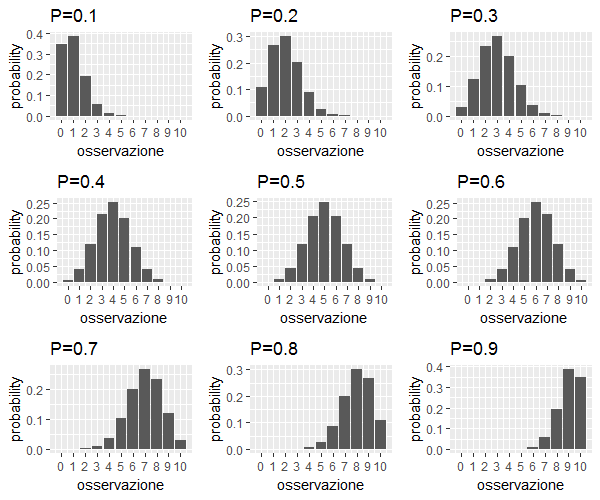
\includegraphics[scale=0.55]{images/dprob.png}
\end{center}
\end{frame}


\begin{frame}{Likelihood-profili di verosimiglianza}

    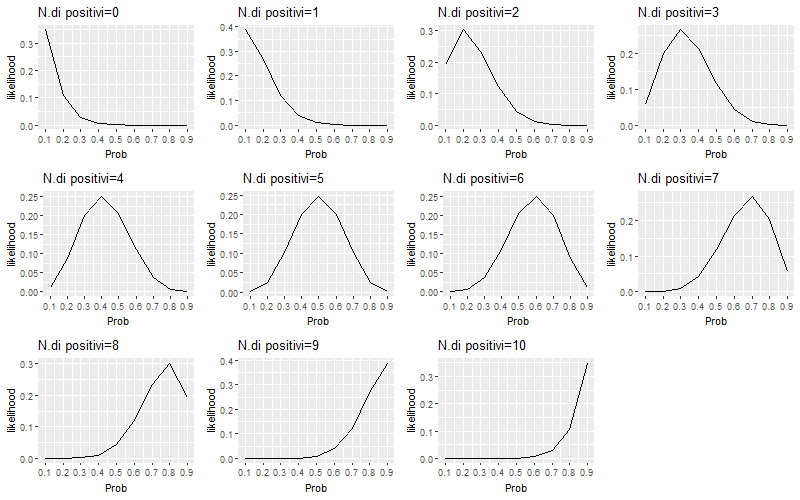
\includegraphics[scale=0.55]{images/lik.png}

\end{frame}




\subsection{metodi induttivi}
\begin{frame}{Teorema di Bayes}
    \begin{columns}
\column{0.3\textwidth}
\begin{center}
    \includegraphics[scale=0.4]{images/bayes.PNG}
\end{center}
\begin{center}
$$P(ipotesi|dati)$$
\end{center}
\column{0.7\textwidth}
\begin{center}
    \textbf{$$P(\theta) \propto Conoscenza x Evidenza$$}
\end{center}
\begin{center}
    \includegraphics[scale=0.2]{images/bayesp.jpg}
\end{center}



\end{columns}
\end{frame}

\begin{frame}{Inferenza bayesiana}
\begin{center}
    \includegraphics[scale=0.53]{images/infbayes.png}
\end{center}
\end{frame}








\section{Strumenti}
\subsection{matrice dati}
\begin{frame}{Frame Title}
    
\end{frame}

\subsection{analisi dei dati con R}
\begin{frame}{Frame Title}
    
\end{frame}

\end{document}